\section{Improving LUT-based architectures}
The LUT networks considered so far were able to learn something, but in order to be viable for real-world ML use, we have to improve the accuracy. Therefore, we now take the idea of LUT networks further and change things to try to improve the accuracy, where we take three main approaches:

\begin{itemize}
  \item modifying existing LUT networks or the LUT network learning algorithm,
  \item enhancing the dataset using feature-engineering and
  \item combining many LUT networks of low bit-sizes (ensembling).
\end{itemize}We will see that we are indeed able to improve the accuracy, where we obtain the best results with an ensembling technique. With an appropriate architecture choice, we are also able to keep model size low.

\subsection{Majority vote} \label{sec:majority_vote}
So far the final prediction came from a single LUT that takes its inputs from the last hidden layer. Considering the same architecture as in the previous section, the last hidden layer has 1024 LUTs. If the number of bits per LUT is eight, then for the final prediction only eight of all 1024 LUTs will be used. Since every LUT is trained with the same label vector $\bm{y}$, each of the 1024 LUTs could theoretically be used for a final prediction too. That motivates us to try a \textit{wisdom of the crowd} technique, a majority vote mechanism that takes into account the predictions of all LUTs in the last hidden layer. The prediction that occurs most often will be chosen as the final one. The complete scheme can be seen in Algorithm~\ref{alg:majority_vote}. We conduct an experiment using a LUT network with five hidden layers and 1024 LUTs per hidden layer, varying the bit-size from two to 10 with steps of one, predicting with and without majority vote each time. The result can be seen in Figure~\ref{fig:majority_vote}. We can see that for a low bit-size, using a majority vote significantly boosts the training and testing accuracy. For high bit-sizes, a majority vote has less effect, but still enhances the testing performance a little. Interestingly, at five bits per LUT all accuracies coincide. Since using a majority vote requires almost no extra computational effort and at worst the results stay the same, it seems to be a good technique for enhancing the network's performance.

\begin{algorithm}
  \caption{LUT network majority vote}
  \label{alg:majority_vote}
  \begin{algorithmic}
    \State Given binary vector $\bm{x}$ and trained LUT network according to Algorithm~\ref{alg:LUT} with $l_L$ LUTs in the last hidden layer, perform a majority vote to predict.
    \vspace{1em}
    \State Initialize empty list $\alpha = [\hspace{0.3em}]$
    \For{$i=1, \dots, j_L$}
      \State Append prediction of LUT$_i$ on $\bm{x}$ to $\alpha$ (either 0 or 1)
    \EndFor
    \If{$\sum\limits_{\alpha_i = 0} > \sum\limits_{\alpha_i = 1}$}
      \State Return 0
    \ElsIf{$\sum\limits_{\alpha_i = 0} < \sum\limits_{\alpha_i = 1}$}
      \State Return 1
    \Else
      \State Return random choice of $\{0, 1\}$
    \EndIf
  \end{algorithmic}
\end{algorithm}
\FloatBarrier

\begin{figure}[!htb]
    \centering
    \includestandalone[]{standalone/lut/majority_vote}
    \caption{Training and testing accuracies with and without using a majority vote mechanism for a LUT network with five hidden layers and 1024 LUTs per hidden layer. The task is Binary-MNIST. For low bit-sizes, using a majority vote significantly enhances performance while the effect lessens with higher bit-sizes, but still enhances the testing accuracy a little. Interestingly, all accuracies coincide at five LUTs per hidden layer.}
\label{fig:majority_vote}
\end{figure}
\FloatBarrier

\subsection{Maximizing layer-wise mean accuracy while training} \label{sec:max_layer_acc}
As mentioned earlier, every LUT is trained with the same label vector $\bm{y}$ and is able to give a prediction. With increasing hidden layer, the LUTs get increasingly better. Figure~\ref{fig:acc_layer_normal} visualizes this using histograms. The underlying data is the training accuracy per LUT per hidden layer for an 8-LUT network with five hidden layers and 1024 LUTs per hidden layer applied on the Binary-MNIST dataset. The training accuracy of this LUT network is 0.89 and the testing accuracy is 0.87, the same accuracies as in the first experiment. The $x$-axis represents the training accuracy. For each hidden layer, we divide the data in 10 equally-sized bins (in terms of the accuracy) from the minimum to maximum value. Then for each bin, we erect a bar, where the height represents the number of data points that fall into this bin. We can see that on average, the accuracy increases with hidden layer number and the spread of accuracies reduces dramatically. For hidden layer 1, the accuracies are worst and the spread is maximal. The worst LUTs on hidden layer 1 are only slightly better than chance. That motivates us to conduct an experiment in which we try to maximize the accuracy of the LUTs while training.

We conceptualize following algorithm: after training a layer, we discard the $n$ worst LUTs in that layer and establish $n$ new LUTs that are hopefully better. We said \enquote{hopefully} because the learning algorithm takes a random subset of columns of the previous layer, leaving it to chance if a new LUT will perform better in terms of accuracy. After obtaining those $n$ new LUTs, we score every LUT and again discard the $n$ worst LUTs until the mean accuracy does not change anymore. We set a patience $p$, i.e., a number of iterations after no change in mean accuracy we will move onto the next layer. The implementation is described in Algorithm~\ref{alg:max_layer_acc}.

\begin{figure}[!htb]
    \centering
    \includestandalone[]{standalone/lut/acc_layer_normal}
    \caption{Histograms of training accuracies per hidden layer for an 8-LUT network with five hidden layers and 1024 LUTs per hidden layer. The task is Binary-MNIST. For each hidden layer, the data is divided into 10 equally sized bins from minimum to maximum value. For each range, we erect a bar with the height equal to the number of data points that fall within that range. The overall accuracy of this network is 0.89 on the training set and 0.87 on the testing set.}
\label{fig:acc_layer_normal}
\end{figure}
\FloatBarrier

\begin{algorithm}
  \caption{Maximizing layer-wise mean accuracy while training}
  \label{alg:max_layer_acc}
  \begin{algorithmic}
    \State Given binary features $\bm{X}$ with $N$ rows and binary label vector $\bm{y}$, construct a LUT network with $L$ hidden layers where the training accuracy in each hidden layer is maximized. This algorithm modifies Algorithm~\ref{alg:LUT}.
    \vspace{1em}
    \State Choose additional hyperparameters:
    \Statein Number of LUTs $n$ to discard after each iteration
    \Statein Patience $p \in \mathds{N}$
    \For{$i = 1, \dots, L$}
      \State Train layer $L$ as in Algorithm~\ref{alg:LUT}
      \State $\text{no\_change} \in \mathds{N} \gets 0$
      \State $\text{best} \in \mathds{R} \gets 0$
      \While{$\text{no\_change} < p$}
      \State Discard $n$ worst performing LUTs on $(\bm{X}, \bm{y})$
      \State Append $n$ new LUTs trained on $(\bm{X}, \bm{y})$ to the current layer
        \State $\text{accs} \in \mathds{R}^N \gets $ accuracy of each LUT on $(\bm{X}, \bm{y})$
        \State $\text{curr} \in \mathds{R} \gets \text{mean}(\text{accs})$
        \If{$\text{curr} > \text{best}$}
          \State $\text{best} \gets \text{curr}$
          \State $\text{no\_change} \gets 0$
          \Else
            \State $\text{no\_change} \mathrel{+}= 1$
        \EndIf
      \EndWhile
    \EndFor
    \State The single LUT after the last hidden layer is created as usual
  \end{algorithmic}
\end{algorithm}
\FloatBarrier

\noindent Starting another experiment, we again use an 8-LUT network with five hidden layers and 1024 LUTs per hidden layer and the Binary-MNIST dataset. We set $p=10$ and $n=50$. After running Algorithm~\ref{alg:max_layer_acc}, we obtain a training accuracy of 0.90 and a testing accuracy of 0.88, slightly better than before. In Figure~\ref{fig:acc_layer_discard} we can see the accuracies per hidden layer visualized using a histogram. Contrary to Figure~\ref{fig:acc_layer_normal}, the distributions are much more narrow now. After training we also tried prediction with a majority vote, but the accuracies did not change.

\begin{figure}[!htb]
    \centering
    \includestandalone[]{standalone/lut/acc_layer_discard}
    \caption{Histograms of training accuracies per hidden layer for an 8-LUT network with five hidden layers and 1024 LUTs per hidden layer, applied on Binary-MNIST. For this network, we applied Algorithm~\ref{alg:max_layer_acc} to try to improve performance, yielding an overall accuracy of 0.90 on the training set and 0.88 on the testing set. The results of this network are slightly better (increase of 1\% training and testing accuracy) compared to the same network without optimization. Contrary to Figure~\ref{fig:acc_layer_normal}, the distributions are much narrower.}
\label{fig:acc_layer_discard}
\end{figure}
\FloatBarrier

\noindent For a more complete picture, we vary the bit-size from two to 10 while applying Algorithm~\ref{alg:max_layer_acc}. There are again five hidden layers with 1024 LUTs per hidden layer. The result can be seen in Figure~\ref{fig:increase_layer_acc}. We can see that pushing up the layer-wise accuracy does indeed help increase the overall accuracy, albeit only significantly for low bit-sizes. For high bit-sizes, the effect is diminished.


\begin{figure}[!htb]
    \centering
    \includestandalone[]{standalone/lut/increase_layer_acc}
    \caption{Training and testing accuracies for LUT networks of varying bit-size with five layers and 1024 LUTs per hidden layer applied on Binary-MNIST. Solid lines and markers denote accuracies of networks where we applied Algorithm~\ref{alg:max_layer_acc}. For low bit-sizes, improving the layer-wise accuracies has a significant effect on the overall performance, while for higher bit-sizes the effect is diminished.}
\label{fig:increase_layer_acc}
\end{figure}
\FloatBarrier

\subsection{Feature engineering} \label{sec:feature_engineering}
So far we have not done any more sophisticated feature engineering except making a binary version out of the original MNIST dataset. Since feature engineering is an integral part of machine learning in general, we try it too and see if there is an improvement of the model's performance. We enhance the data by emphasizing the edges. Concretely, we create a copy of the original image and replace each pixel with black if the adjacent pixel has the same value and white if the adjacent pixel has a different value. We do this process both in $x$- and $y$-direction and add the results to the original image. Figure~\ref{fig:sobel_single} illustrates this technique for one example.

\begin{figure}[!htb]
    \centering
    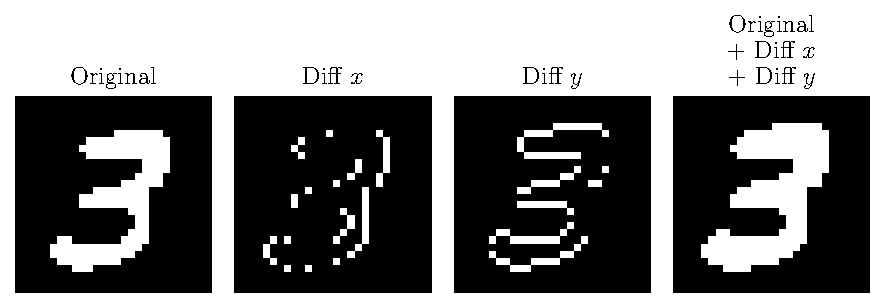
\includegraphics[width=.9\linewidth]{images/diff.pdf}
    \caption{Single example from the training data where we applied feature engineering. We create a copy of the original image and replace each pixel with black if the adjacent pixel has the same value and white if the adjacent pixel has a different value. We perform this process both in $x$- and $y$-direction and add the results to the original image. Looking at the feature-engineered image on the right, the number appears thicker.}
\label{fig:sobel_single}
\end{figure}
\FloatBarrier

\noindent Using the dataset enhanced with feature engineering, we train a LUT network with five hidden layers and 1024 LUTs per hidden layer, varying the bit-size from two to 10. The result can be seen in Figure~\ref{fig:sobel_acc}. We can see that the accuracies are consistently higher for models that were trained on images where feature engineering had been applied. The technique described in this section was inspired by the Sobel operator \cite{bib:sobelsobel} which calculates the gradients in an image in either $x$- or $y$-direction. Using this operator as feature engineering technique as opposed to our own produces similar results. We presented our own as main technique for the sake of an easier explanation and brevity.

\begin{figure}[!htb]
    \centering
    \includestandalone[]{standalone/lut/feature_engineering}
    \caption{Train and test accuracies for models trained on unmodified Binary-MNIST data and Binary-MNIST data where feature engineering had been applied. We can see that using feature engineering boosts the performance slightly.}
\label{fig:sobel_acc}
\end{figure}
\FloatBarrier


\subsection{Plain LUT ensembling} \label{sec:plain_lut_ensemble}
In Section~\ref{sec:majority_vote}, as opposed to having one final LUT, we counted the number of output labels in the last hidden layer and took that label as final prediction whichever was occurring the most. We could view that as a \textit{wisdom of the crowd} technique. Another approach is to bunch together $n$ separate LUT networks that do not use a majority vote and combine their prediction into one. We simply use that label as final prediction which was predicted the most out of the $n$ LUT networks. In the event that both labels occur the same number of times, we make a random choice. The scheme is described in detail in Algorithm~\ref{alg:lut_ensemble}.

We conduct an ensembling experiment where we use 2-LUTs as base classifiers. Keeping the bit-size low allows us to increase the number of individual LUT networks to a much higher degree. Training and inference for 8-LUT networks would take too long, at least with our current code. Figure~\ref{fig:plain_lut_ensembling} visualizes the result of the experiment. We use LUT network ensembles with $2^{1, \dots, 10}$ individual LUT classifiers. At just two LUT networks, the training accuracy is fairly low at 0.68, as it would be with a single 2-LUT network. Increasing the number of LUT networks increases the training accuracy and a peak at 0.78 with 64 LUTs is reached. Increasing the number of LUTs even more has no effect on the accuracy. Interestingly, the testing accuracy is consistently higher than the training accuracy.

\begin{algorithm}
  \caption{LUT ensembling}
  \label{alg:lut_ensemble}
  \begin{algorithmic}
    \State Given trained $\text{LUT}_{1, \dots, n}$, perform ensembling to predict on yet unseen $\bm{x}$.
    \vspace{1em}
    \State Initialize empty list $\alpha = [\hspace{0.3em}]$
    \For{$i=1, \dots, n$}
      \State Append prediction of LUT$_i$ on $\bm{x}$ to $\alpha$ (either 0 or 1)
    \EndFor
    \If{$\sum\limits_{\alpha_i = 0} > \sum\limits_{\alpha_i = 1}$}
      \State Return 0
    \ElsIf{$\sum\limits_{\alpha_i = 0} < \sum\limits_{\alpha_i = 1}$}
      \State Return 1
    \Else
      \State Return random choice of $\{0, 1\}$
    \EndIf
  \end{algorithmic}
\end{algorithm}
\FloatBarrier

\begin{figure}[!htb]
    \centering
    \includestandalone[]{standalone/lut/plain_lut_ensembling}
    \caption{Train and test accuracies for LUT network ensembles according to Algorithm~\ref{alg:lut_ensemble} on Binary-MNIST. The base classifiers are 2-LUT networks with five hidden layers and 1024 LUTs per hidden layer. Training and testing accuracies reach a peak at 64 LUT networks, increasing the LUT number even more has no effect on the accuracy. Interestingly, the testing accuracy is consistently higher than the training accuracy.}
\label{fig:plain_lut_ensembling}
\end{figure}
\FloatBarrier

\subsection{Advanced LUT ensembling} \label{sec:ada_boost}
Now we try another ensembling method which is very well established in literature and practice, the AdaBoost.M1 algorithm \cite{bib:adaboostm1} which can be seen in Algorithm~\ref{alg:adaboostm1}. As the scheme in the previous Section~\ref{sec:plain_lut_ensemble}, AdaBoost.M1 combines predictions of $n$ separate classifiers $f_{1, \dots, n}$ into one. Every classifier is trained individually with the addition of weights $\bm{w}$, where $w_k > 0$. Every sample $k$ in the training set is assigned weight $w_k = 1/N$ in the beginning, where $N$ is the number of samples. The weights represent how much attention during training a single example should get, the higher the weight, the more attention the sample gets. Since all weights are equal in the beginning, every sample gets the same amount of attention in the first iteration. Once iteration $i$ is finished, a number $\alpha_i \in \mathds{R}$ is computed. If $\alpha_i > 0$, then the classifier is better than random and if $\alpha_i < 0$, then the classifier is worse than random. Using $\alpha_i$, we update each weight of only those samples which were misclassified. If the classifier is better than random, then we can do some fine-tuning and focus more on the misclassifications which corresponds to assigning higher weights to misclassified samples. If the classifier is worse than random, then we are not yet ready for fine-tuning and we should focus more on the most important samples which corresponds to assigning lower weights to misclassified samples. After $n$ iterations, training is finished and we can predict on yet unseen sample $\bm{x}$ using $\text{sign}(\sum_{i=1}^n \alpha_i f_i(\bm{x}))$. 

\begin{algorithm}
  \caption{AdaBoost.M1 algorithm according to \cite{bib:adaboostm1}} \label{alg:adaboostm1}
  \begin{algorithmic}[1]
    \State Given dataset $(\bm{X}, \bm{y})$, where $\bm{X} = \bm{x}_1, \dots, \bm{x}_N$ and $\bm{y} = y_1, \dots, y_N$, $y_i \in \{-1, 1\}$ and model class, construct a classifier that is made up of $n$ individual classifiers $f_1, \dots, f_n$.
    \vspace{1em}
    \State Initialize weight vector $\bm{w} \in \mathds{R}^N$ with $w_{1, \dots, N} = 1/N$
    \vspace{0.5em}
    \For{$i = 1, \dots, n$}
    \State Train classifier $f_i$ on $(\bm{X},\bm{y})$ and weights $\bm{w}$ \label{alg_line:adaboostm1:train}
    \State $\text{err}_i \gets \big( \sum_{k=1}^N w_k \mathbb{1}(f_i(\bm{x}_k) \neq y_k) \big) / \sum_{k=1}^N w_k$
    \State $\alpha_i = \log((1 - \text{err}_i) / \text{err}_i)$
    \For{$k = 1, \dots, N$}
    \State $w_k \gets w_k \exp(\alpha_i \mathbb{1}(f_i(\bm{x}_k) \neq y_k))$
    \EndFor
    \EndFor
    \State Prediction on yet unseen $\bm{x}$: $\text{sign} \big( \sum_{i = 1}^n \alpha_i f_i(\bm{x}) \big)$
  \end{algorithmic}
\end{algorithm}
\FloatBarrier

\noindent Using AdaBoost.M1 with LUT networks only works if we modify the algorithm slightly. Looking at Algorithm~\ref{alg:adaboostm1} on line~\ref{alg_line:adaboostm1:train}, we notice that there is no way to incorporate weights into the LUT learning algorithm (see Algorithm~\ref{alg:LUT}). Therefore, instead of training on all samples $\bm{X}$ with weights at each iteration, we train on a subset of samples $\bm{X}' \subset \bm{X}$ with fixed size $\rho \in \{1, \dots, N\}$ without weights. By choosing those samples with highest weights to be included in $\bm{X}'$, we are able to give more attention to those samples. The modified AdaBoost.M1 for LUT networks can be seen in Algorithm~\ref{alg:lut_ensemble_ada}. The modifications take place from line~\ref{alg_ref:lut_ensemble_ada:mod_begin} to line~\ref{alg_ref:lut_ensemble_ada:mod_end}. On the first iteration, we train on the entire dataset. On all other iterations, we train on $\rho$ samples with the highest weights. The command $\text{argsort}(\bm{w})$ returns indices that would sort $\bm{w}$. We are interested in the highest weights, not the lowest ones, so we reverse the sorted indices: $\text{reversed}(\text{argsort}(\bm{w}))$. We then take a subset, the first $\rho$ entries: $\text{reversed}(\text{argsort}(\bm{w}))[:\rho]$. Now we have the indices of $\rho$ samples with highest weights and take a subset of the dataset: $\bm{X}[\text{idxs}]$ and $\bm{y}[\text{idxs}]$.

\begin{algorithm}
  \caption{LUT ensembling inspired by AdaBoost.M1}\label{alg:lut_ensemble_ada}
  \begin{algorithmic}[1]
    \State Given dataset $(\bm{X}, \bm{y})$, where $\bm{X} = \bm{x}_1, \dots, \bm{x}_N$ and $\bm{y} = y_1, \dots, y_N$, $y_i \in \{-1, 1\}$, construct a classifier that is made up of $n$ individual classifiers $\text{LUT}_{1, \dots, n}$.
    \vspace{1em}
    \State Initialize weight vector $\bm{w} \in \mathds{R}^N$ with $w_{1, \dots, N} = 1/N$
    \State Choose $\rho$ out of $\{1, \dots, N\}$
    \vspace{0.5em}
    \For{$i = 1, \dots, n$} \label{alg_ref:lut_ensemble_ada:mod_begin}
    \If{i = 1}
      \State Train $\text{LUT}_i$ on $(\bm{X},\bm{y})$
    \Else
    \State $\text{idxs} = \text{reversed}(\text{argsort}(\bm{w}))[:\rho]$
    \State $\bm{X}' \subset \bm{X} \gets \bm{X}[\text{idxs}]$
    \State $\bm{y}' \subset \bm{y} \gets \bm{y}[\text{idxs}]$
      \State Train $\text{LUT}_i$ on $(\bm{X}', \bm{y}')$
      \EndIf \label{alg_ref:lut_ensemble_ada:mod_end}
    \State $\text{err}_i \gets \big( \sum_{k=1}^N w_k \mathbb{1}(\text{LUT}_i(\bm{x}_k) \neq y_k) \big) / \sum_{k=1}^N w_k$
    \State $\alpha_i = \log((1 - \text{err}_i) / \text{err}_i)$
    \For{$k = 1, \dots, N$}
    \State $w_k \gets w_k \exp(\alpha_i \mathbb{1}(\text{LUT}_i(\bm{x}_k) \neq y_k))$
    \EndFor
    \EndFor
    \State Prediction on yet unseen $\bm{x}$: $\text{sign} \big( \sum_{i = 1}^n \alpha_i \text{LUT}_i(\bm{x}) \big)$
  \end{algorithmic}
\end{algorithm}
\FloatBarrier

\noindent We apply Algorithm~\ref{alg:lut_ensemble_ada} and use 2-LUT networks with five hidden layers and 1024 LUTs per hidden layer and choose $\rho = N/5$. We vary the number of LUT networks from 2 to 1024. The motivation for choosing 2-LUT networks is computation time and disk size. Since we want to keep open the possibility for many LUT networks in the ensembled classifier, we have to restrict ourselves with the bit-size, otherwise it would take too long to train and predict. Our overall goal also includes a small disk size. A LUT network ensemble of 8-LUTs with five hidden layers and 1024 LUTS per hidden layer would take up 168 MB of space, way out of proportions. The results can be seen in Figure~\ref{fig:ada_2_LUT}. We can see that with an increasing number of LUT networks, we can indeed improve the accuracy. At 1024 LUT networks, we achieve a training accuracy of 0.94 and testing accuracy of 0.93. When it comes to the testing accuracy, this is the best result so far. Interesting is the lack of a significant difference between training and testing accuracies. Usually there is a point where overfitting starts to take place and the testing accuracy decreases compared to the training accuracy. Perhaps overfitting will take place at more LUT networks than 1024, but we do not go above that because it would take too much time to train for us. However, a LUT network ensemble of 2-LUTs with five hidden layers and 1024 LUTs per hidden layer takes up 2.62 MB of disk space, larger than the CNN we used before which was 1.16 MB in size. We therefore evaluate training and testing performance on a 2-LUT ensemble with five hidden layers and only 64 LUTs per hidden layer. This architecture takes up only 168 KB of disk space. We obtain a trainig and testing accuracy of 0.94.

\begin{figure}[!htb]
    \centering
    \includestandalone[]{standalone/lut/ada_2_LUT}
    \caption{Training and testing accuracies for ensembles of 2-LUT networks with five hidden layers and 1024 LUTs per hidden layer according to Algorithm~\ref{alg:lut_ensemble_ada}. At 1024 LUT networks, we obtain training and testing accuracies of 0.94 and 0.93, respectively, best so far when it comes to testing accuracy. Notice the lack of significant difference between training and testing accuracy as it would be when overfitting. Perhaps overfitting takes place at more individual LUTs. Using 1024 LUT networks per hidden layer make the size of this ensemble be 2.62 MB which is bigger than the CNN with 1.16 MB we used before. Performing another experiment with an ensemble of 1024 2-LUT networks with five hidden layers and only 64 LUTs per hidden layer, we obtain a training and testing accuracy of 0.94 and this architecture only takes up 168 KB of space.}
\label{fig:ada_2_LUT}
\end{figure}
\FloatBarrier

\noindent As opposed to LUT architectures in previous sections, the AdaBoost.M1 inspired ensemble requires floating-point computations to make predictions ($\alpha_i$ in Algorithm~\ref{alg:lut_ensemble_ada}). LUTs and LUT networks can be implemented fast on a binary level, since for inference, we just have to look up entries in tables. The floating-point computation here further complexifies inference, however, we will not investigate to what degree speed is influenced.

\subsection{Combining different methods}
We combine different methods presented in previous sections to try to push the accuracies even further. We utilize an AdaBoost.M1 inspired LUT classifier from Section~\ref{sec:ada_boost} with 1024 individual 2-LUT networks that each have 5 hidden layers and 64 LUTs per hidden layer. Additionally, we apply Algorithm~\ref{alg:max_layer_acc} to each LUT network while training and also use the feature-engineered dataset from Section~\ref{sec:feature_engineering}. For the hyperparameters, we set $\rho = N/5$, the number of LUTs to discard after each iteration $n=10$ and patience $p=10$. We obtain a training accuracy of 0.75 and testing accuracy of 0.78, worse than the results from Section~\ref{sec:ada_boost}. The results make us question Algorithm~\ref{alg:max_layer_acc}. It is interesting though that pushing up the accuracies of individual LUTs in LUT networks leads to an overall inferior performance when constructing an ensembled classifier.

\subsection{Summary}
Starting with a LUT-network architecture from \cite{bib:chatterjee2018learning}, we tried to make improvements in terms of accuracy and size which were successful. A majority vote and maximizing the layer-wise mean accuracy while training help improving performance of single LUT networks of low bit-size, for higher bit-sizes, however, the change does not surpass 1-2\%. Feature engineering gave small improvements in accuracy. Ensembling techniques are promising, especially an AdaBoost.M1 ensemble achieved a testing accuracy of 0.94, better than any previous single LUT networks. With a good choice of architecture, we were able to reduce the size of the ensemble significantly while retaining accuracy. However, the advance ensembling scheme requires floating-point computations again, albeit few. We also obtained results that suggest combining ensembling and maximizing the layer-wise mean accuracy is not a good idea. What we have not discussed is pruning of LUT networks, i.e. discarding individual LUTs that do not contribute to the final prediction. We have also not discussed multi-class classification which would be possible with LUTs using an one-vs-one or one-vs-all approach similar to SVMs \cite{bib:bishop2006pattern}.
